\chapter{\texorpdfstring{Free-Choice Nets}{Free-Choice Nets}}
\label{ch:17}
\lecturemeta{Lezione 17 \quad\textbullet\quad 2026-07-04 \quad\textbullet\quad Roberto Bruni}{Esparza, \emph{Free Choice Petri Nets}}

Nelle traduzioni di \hyperref[ch:16a]{EPC} e \hyperref[ch:16b]{BPMN} è emersa una classe ricorrente: i \textbf{free-choice net}. Sono più generali degli \hyperref[ch:15]{S-net e T-net} ma conservano proprietà strutturali bellissime. Questa lezione le studia, arrivando a due risultati profondi: la \textbf{liveness} di un free-choice net è caratterizzabile con siphon e trap (\textbf{teorema di Commoner}), ma è \textbf{NP-complete} da decidere; mentre \textbf{liveness + boundedness} insieme si decidono in \textbf{tempo polinomiale} (\textbf{Rank Theorem}). Sono i concetti di \hyperref[ch:17aux]{17aux — P and NP} applicati alle reti.

\section{\texorpdfstring{La motivazione: separare scelta e sincronizzazione}{La motivazione: separare scelta e sincronizzazione}}

Il problema che vogliamo eliminare è l'\textbf{interferenza fra conflitto e sincronizzazione}. In una rete qualsiasi due transizioni $t_1, t_2$ possono essere inizialmente indipendenti e diventare in conflitto dopo che una \emph{terza} transizione $t_3$ scatta — e lo scatto di $t_3$ non è controllabile. La scelta fra $t_1$ e $t_2$ finisce così per dipendere dal resto del sistema.

L'idea dei free-choice è \textbf{impedire} che una scelta fra transizioni sia influenzata da altro. Il modo più semplice: tenere \textbf{separati} i place con più transizioni uscenti dalle transizioni con più place entranti.

\begin{boxdefinition}{Free-choice net — idea intuitiva (versione forte)}
Il modo più semplice per capire l'obiettivo: per ogni arco $(p,t)$, deve valere almeno una di: - $t$ è l'\textbf{unica} transizione uscente da $p$ ($|p\bullet| = 1$, nessun conflitto su $p$), \textbf{oppure} - $p$ è l'\textbf{unico} place entrante in $t$ ($|\bullet t| = 1$, nessuna sincronizzazione su $t$).

Questa è solo l'idea guida, \textbf{non} la definizione ufficiale: è più restrittiva di quella che useremo (esclude anche casi che vorremmo ammettere, come due transizioni che condividono \emph{più} place di input).
\end{boxdefinition}

\begin{boxdefinition}{Free-choice net (definizione ufficiale)}
Un Petri net è \textbf{free-choice} se, per ogni coppia di \textbf{transizioni}, i loro \textbf{pre-set} sono \textbf{disgiunti oppure uguali}: \(\forall t, t' \in T.\quad \bullet t \cap \bullet t' = \emptyset \;\lor\; \bullet t = \bullet t'\) Equivalentemente (dualmente), per ogni coppia di \textbf{place}, i loro \textbf{post-set} sono disgiunti oppure uguali.

Un system $(N, M_0)$ è free-choice se $N$ lo è.

Questa condizione è \textbf{più debole} (ammette più reti) della versione intuitiva sopra: qui due transizioni possono benissimo condividere \emph{due o più} place di input, purché li condividano \emph{tutti} — non serve che il pre-set sia un singoletto.
\end{boxdefinition}

L'intuizione della definizione ufficiale: se due transizioni condividono \emph{anche un solo} place di input, allora devono condividerli \emph{tutti} — così sono sempre abilitate insieme, e la scelta fra loro è davvero \textbf{libera} (dipende solo dai token in quei place comuni, non da altro).

\begin{figure}[!htb]
\centering
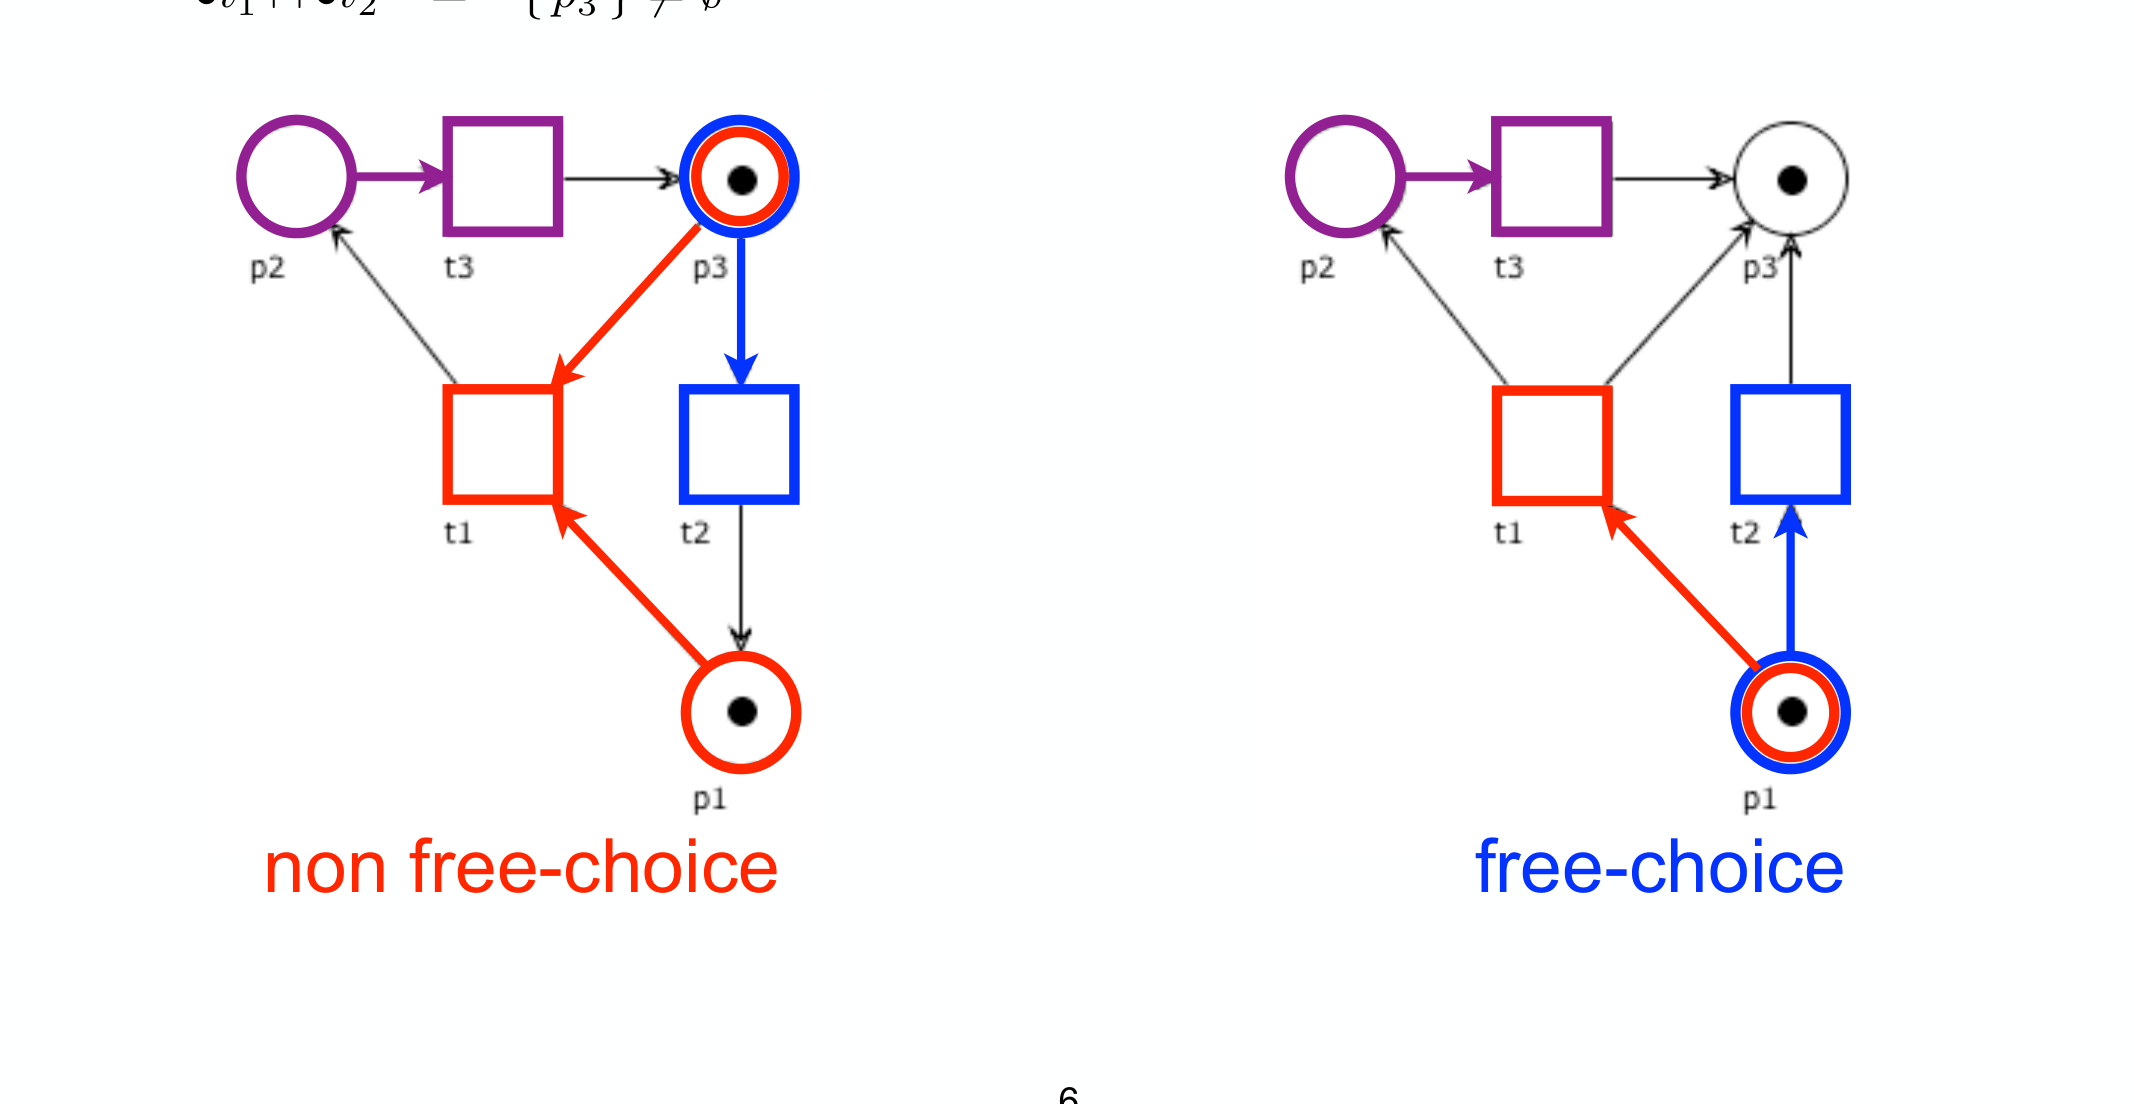
\includegraphics[width=0.74\linewidth,height=0.34\textheight,keepaspectratio]{images/17-free-choice_p6_fc-vs-nonfc.png}
\caption{Sinistra: \textbf{non} free-choice, perché $\bullet t_1 = \{p_1,p_3\}$ e $\bullet t_2 = \{p_3\}$ si intersecano in $p_3$ ma non coincidono. Destra: free-choice, perché $\bullet t_1 = \bullet t_2$ e $\bullet t_3$ è disgiunto da entrambi.}
\end{figure}

\begin{boxnote}{S-net e T-net sono free-choice}
\begin{itemize}
\item Ogni \textbf{S-net} è free-choice: in un S-net ogni $\bullet t$ è un \textbf{singoletto}, quindi due pre-set o coincidono o sono disgiunti.
\item Ogni \textbf{T-net} è free-choice: in un T-net ogni $p\bullet$ è un singoletto, stesso ragionamento sui post-set.
\end{itemize}

I free-choice sono dunque una \textbf{super-classe} comune di S-net e T-net (e la contengono strettamente: esistono free-choice che non sono né l'uno né l'altro).
\end{boxnote}

La proprietà che dà il nome alla classe:

\begin{boxtheorem}{Proprietà fondamentale dei free-choice}
Se $M$ abilita $t$ e $t \in p\bullet$, allora $M$ abilita \textbf{ogni} $t' \in p\bullet$.

\emph{Perché:} in un free-choice $t, t' \in p\bullet$ implica $\bullet t = \bullet t'$, quindi se i place comuni bastano per $t$ bastano anche per $t'$. La scelta fra le transizioni che escono da $p$ è \textbf{libera}: o sono tutte abilitate, o nessuna lo è.
\end{boxtheorem}

Come per la soundness, ci interessa la trasformata $N^\star$ (che aggiunge la transizione reset $o \to i$):

\begin{boxnote}{$N$ free-choice $\iff$ $N^\star$ free-choice}
$N$ e $N^\star$ differiscono solo per la transizione \textbf{reset}, il cui pre-set $\{o\}$ è disgiunto dal pre-set di ogni altra transizione. Aggiungere reset non rompe la proprietà free-choice.
\end{boxnote}

\section{\texorpdfstring{Liveness = place-liveness}{Liveness = place-liveness}}

Un primo regalo dei free-choice riguarda la liveness. In \emph{qualsiasi} rete, la liveness implica la \textbf{place-liveness} (nessun place può diventare "morto", cioè permanentemente inutilizzabile): se un place $p$ è dead, ogni transizione nel suo pre/post-set è dead. Nei free-choice vale anche il \textbf{viceversa}.

\begin{boxtheorem}{Liveness = place-liveness (free-choice)}
In un free-choice system: \textbf{place-live $\iff$ live}.

\emph{Intuizione ($\Rightarrow$):} per abilitare una transizione $t$ con $\bullet t = \{p_1, \dots, p_n\}$ partendo da una marcatura $M$, si costruisce la catena, sfruttando ogni volta la place-liveness:

\[
M \ \leadsto\ M_1 \ (\text{marca } p_1) \ \leadsto\ M_2 \ (\text{marca } p_2) \ \leadsto\ \dots \ \leadsto\ M_n \ (\text{marca } p_n)
\]

Il punto delicato è che \textbf{i token già messi non si perdono}: per la proprietà fondamentale, se una $t'$ potesse togliere il token da $p_1$, avrebbe lo stesso pre-set di $t$ — ma allora abiliterebbe direttamente $t$. Alla fine $M_n$ marca tutti i $p_i$ e \textbf{abilita $t$}.
\end{boxtheorem}

\begin{figure}[!htb]
\centering
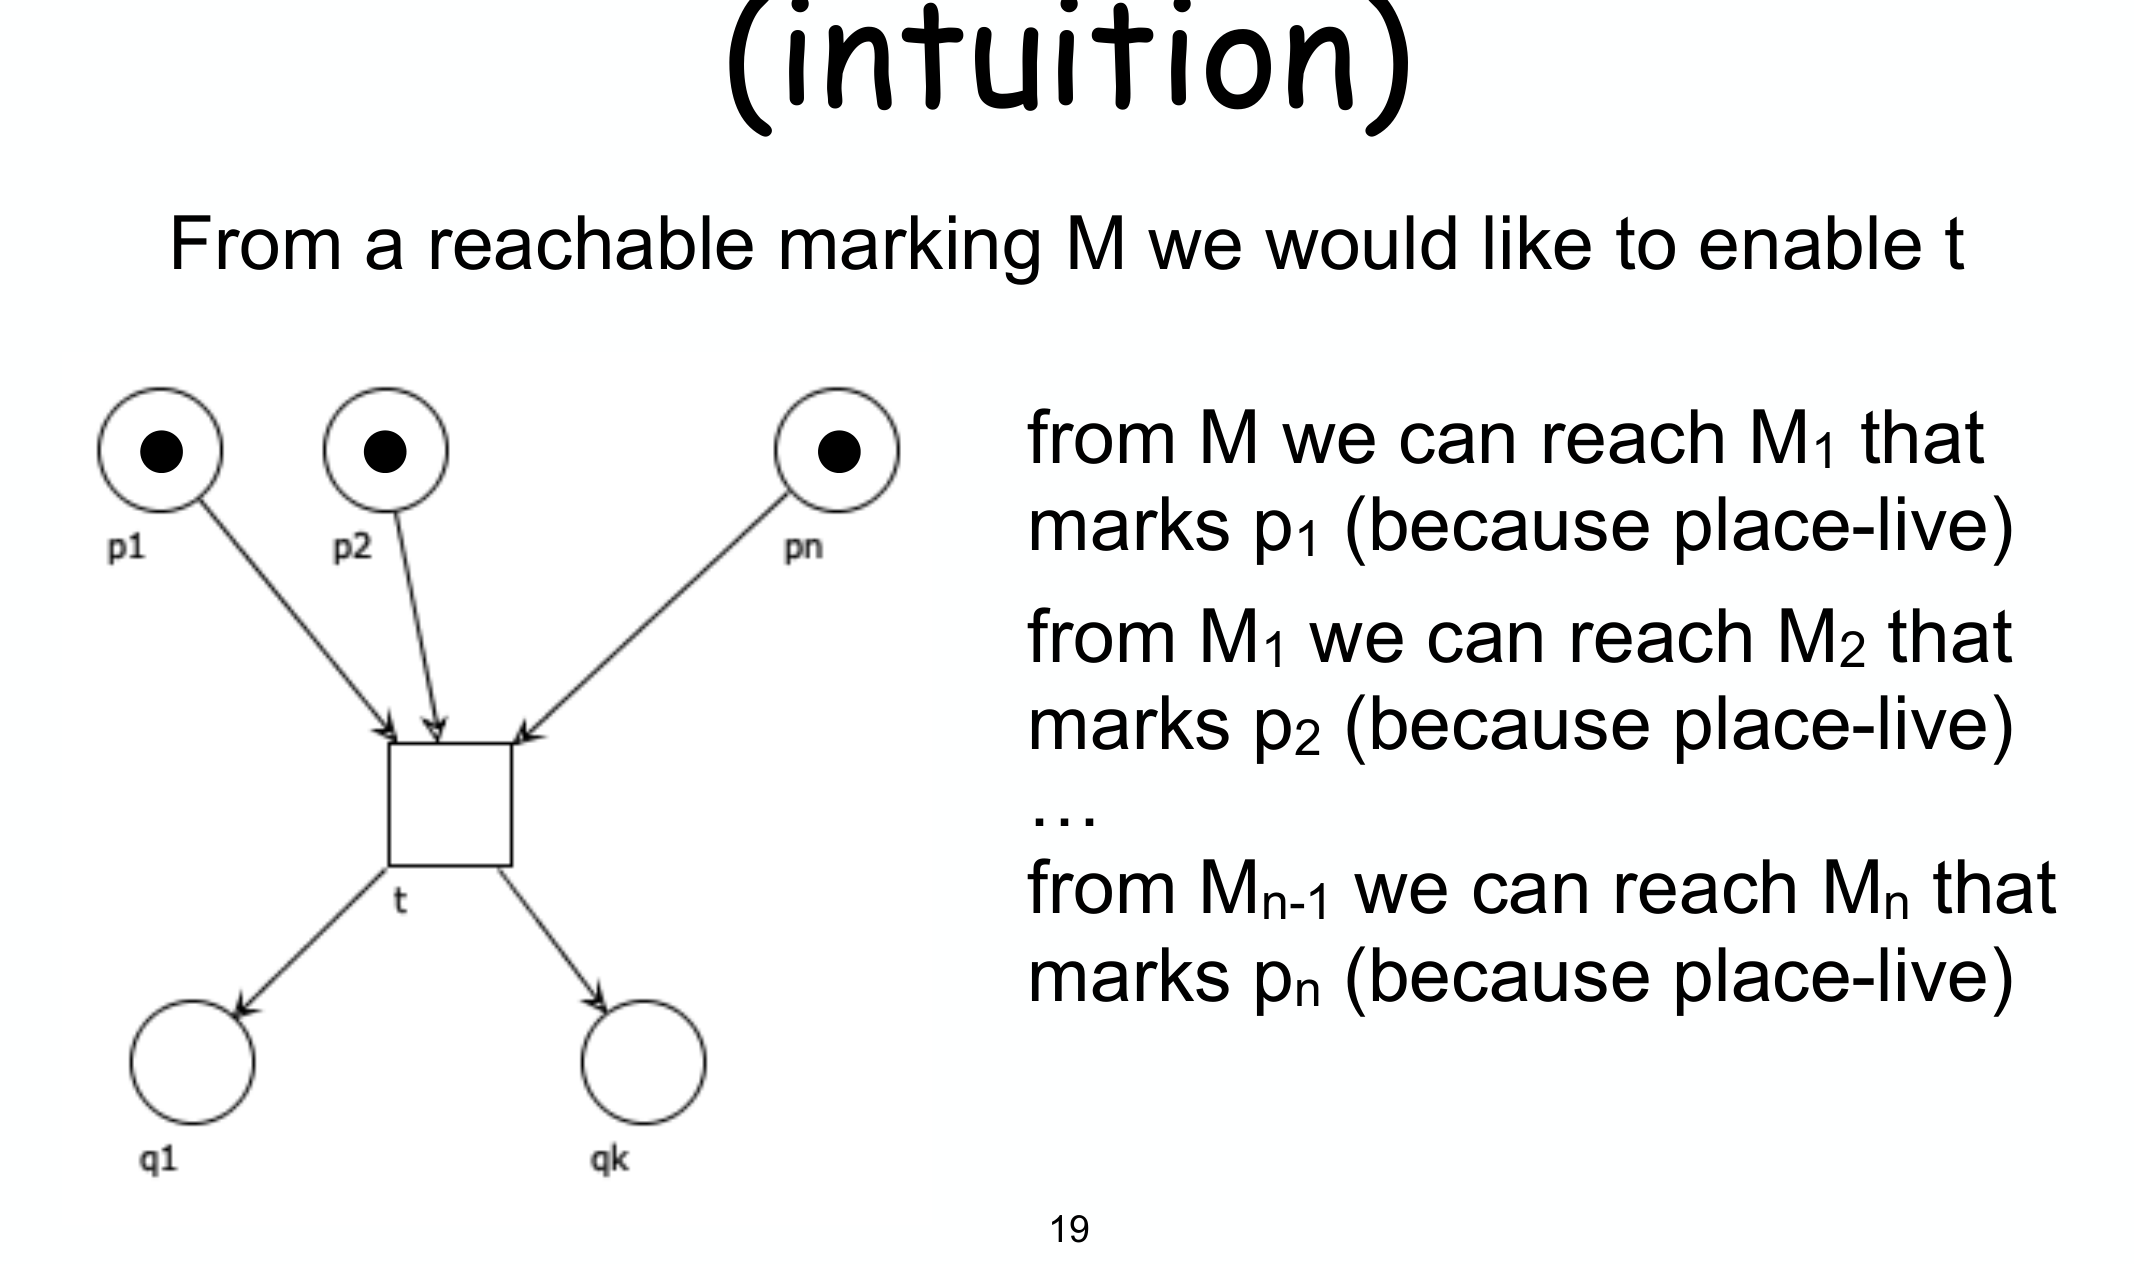
\includegraphics[width=0.74\linewidth,height=0.34\textheight,keepaspectratio]{images/17-free-choice_p19_place-live-intuition.png}
\caption{La costruzione passo-passo: si marca \textbf{un place di input alla volta} ($p_1$, poi $p_2$, …, poi $p_n$), sfruttando ogni volta la place-liveness. Il passaggio delicato (non visibile nel disegno, ma cruciale) è che marcare $p_2$ non deve "svuotare" $p_1$: qui interviene la proprietà fondamentale dei free-choice, che impedisce a un'altra transizione di rubare il token da $p_1$ senza condividerne l'intero pre-set con $t$.}
\end{figure}

\section{\texorpdfstring{Siphon e trap}{Siphon e trap}}

Il cuore tecnico della lezione sono due strutture duali sui place: i \textbf{siphon} (che, una volta svuotati, restano vuoti) e i \textbf{trap} (che, una volta marcati, restano marcati). Servono a fissare le "trappole" strutturali della liveness. Conviene prima l'idea, poi la formula.

\begin{boxdefinition}{Siphon (o deadlock)}
Un insieme di place $R$ è un \textbf{siphon} se ogni transizione che può \textbf{produrre} token in $R$ richiede anche un place di $R$ come input: $\;\bullet R \subseteq R\bullet$.

\textbf{Conseguenza:} se $R$ è \textbf{vuoto} (nessun token), nessuna transizione potrà mai rimetterci token $\rightarrow$ \textbf{resta vuoto per sempre}. È \textbf{proper} se $R \ne \emptyset$.
\end{boxdefinition}

\begin{boxdefinition}{Trap}
Un insieme di place $R$ è un \textbf{trap} se ogni transizione che può \textbf{consumare} token da $R$ produce anche un token in $R$: $\;R\bullet \subseteq \bullet R$ (scritto anche $\bullet R \supseteq R\bullet$).

\textbf{Conseguenza:} se $R$ è \textbf{marcato} (almeno un token), non potrà mai svuotarsi $\rightarrow$ \textbf{resta marcato per sempre}. È \textbf{proper} se $R \ne \emptyset$.
\end{boxdefinition}

La lettura "meccanica" è comoda: un siphon controlla che $\bullet R$ (frecce \emph{entranti} in $R$) sia coperto da $R\bullet$ (frecce \emph{uscenti}); un trap è l'inclusione opposta.

\begin{figure}[!htb]
\centering
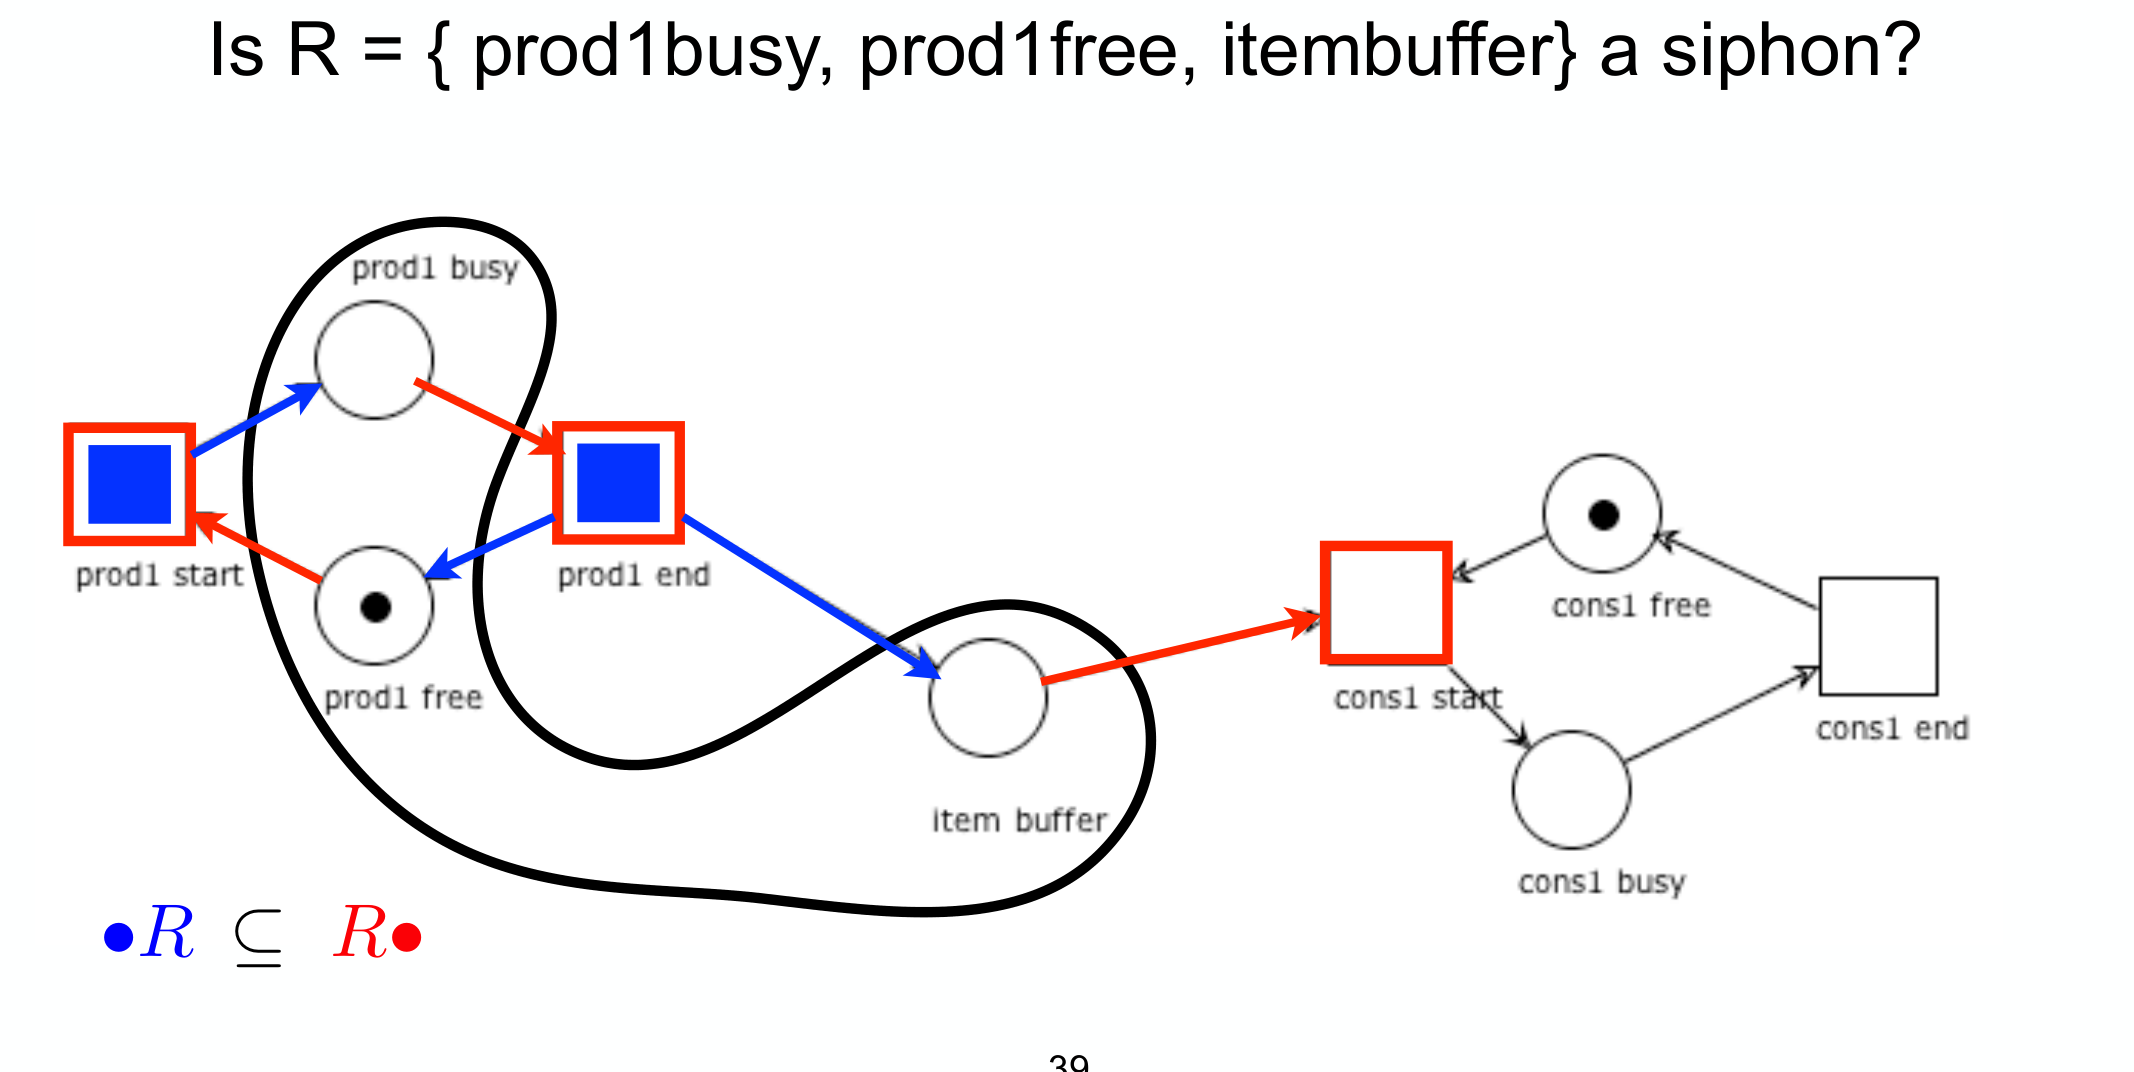
\includegraphics[width=0.74\linewidth,height=0.34\textheight,keepaspectratio]{images/17-free-choice_p39_siphon-check.png}
\caption{Verifica siphon: si colora $\bullet R$ (transizioni che entrano in $R$) e $R\bullet$ (transizioni che escono). $R$ è un siphon sse $\bullet R \subseteq R\bullet$.}
\end{figure}

\begin{figure}[!htb]
\centering
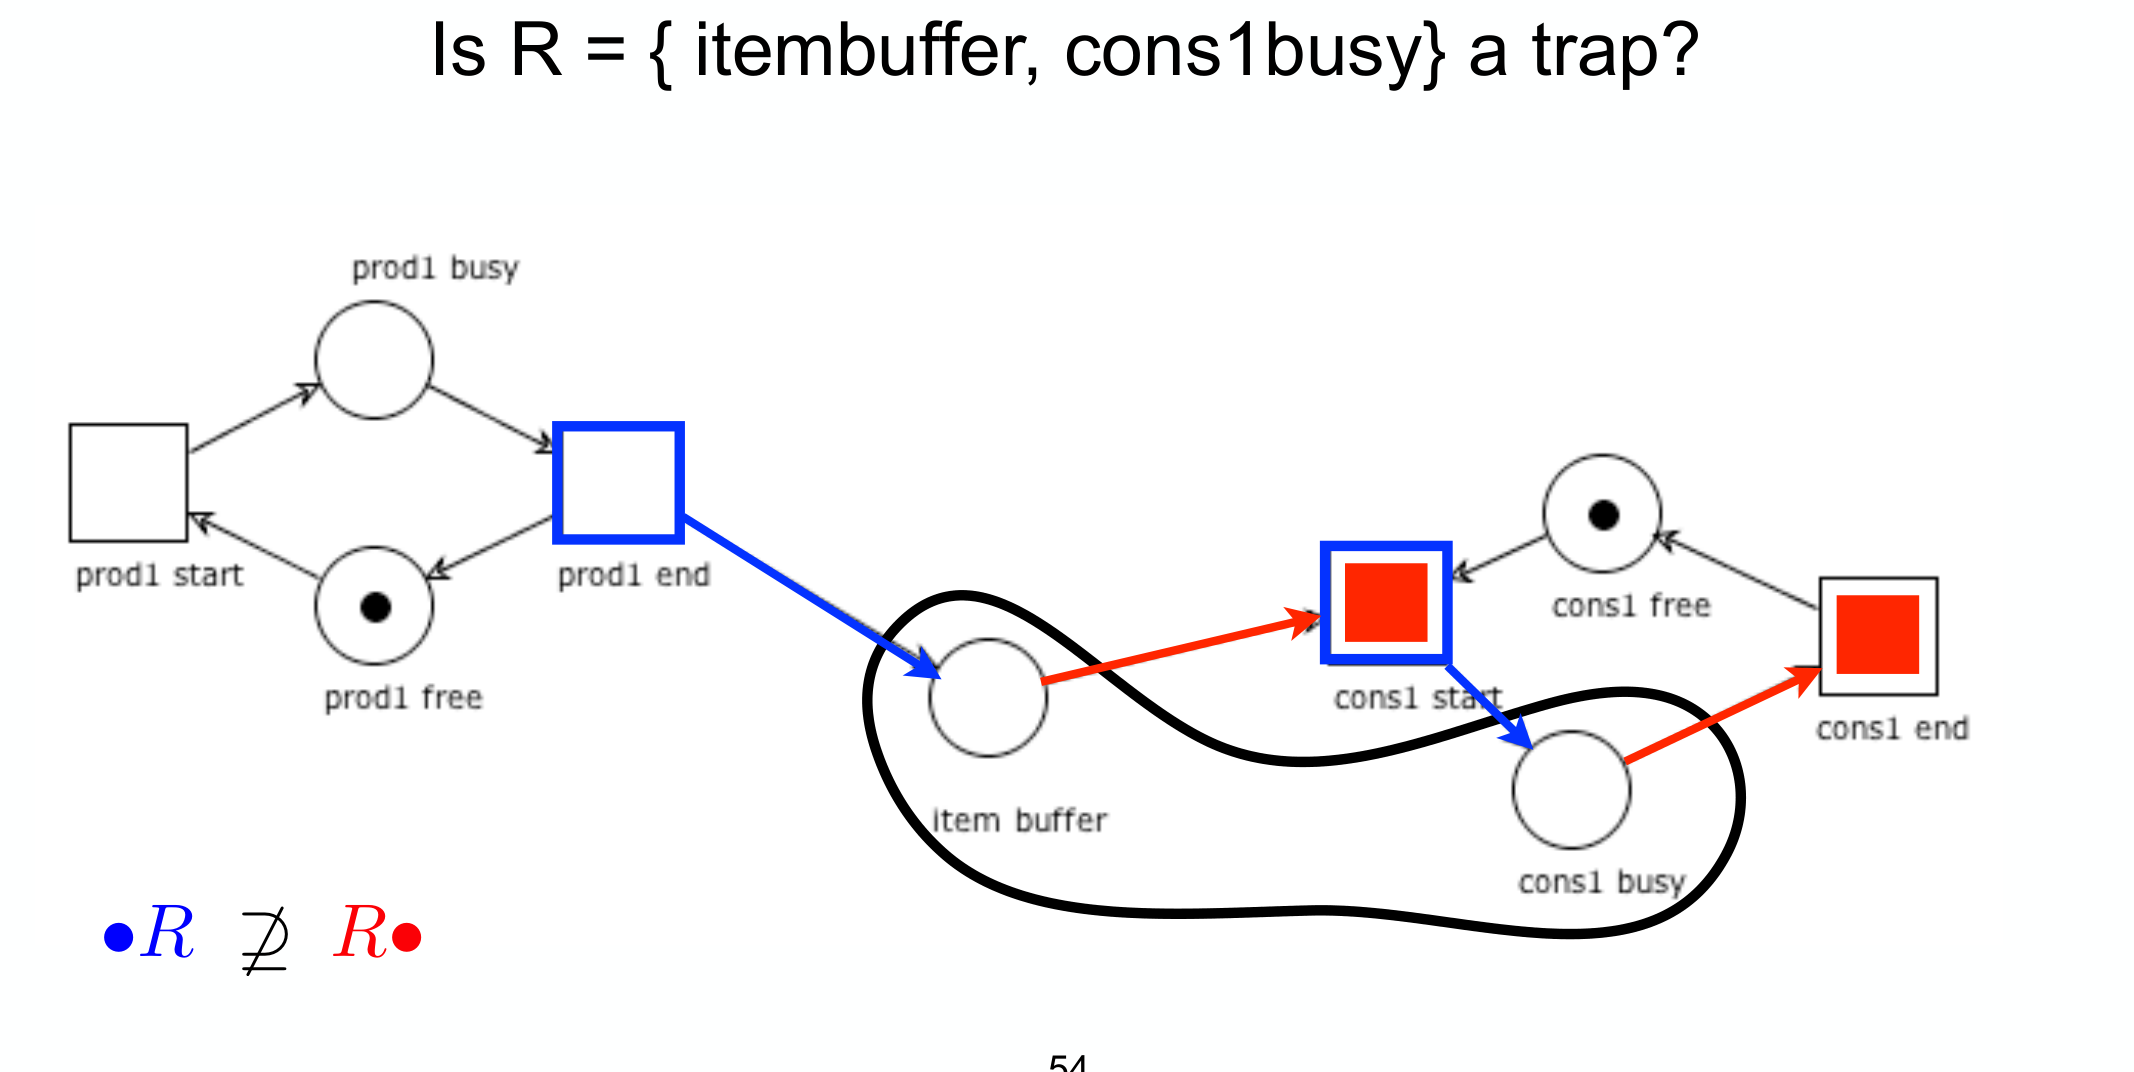
\includegraphics[width=0.74\linewidth,height=0.34\textheight,keepaspectratio]{images/17-free-choice_p54_trap-check.png}
\caption{Verifica trap: qui $R\bullet \not\subseteq \bullet R$, quindi $R = \{\text{itembuffer}, \text{cons1busy}\}$ \textbf{non} è un trap.}
\end{figure}

Queste "conseguenze" si formalizzano con la nozione di \textbf{stable set of markings}: un insieme $\mathcal{M}$ di marcature è \textbf{stable} se, partendo da una qualsiasi marcatura in $\mathcal{M}$, non si può raggiungere una marcatura fuori da $\mathcal{M}$. Le proprietà fondamentali di siphon e trap dicono esattamente che certi insiemi sono stable:

\begin{boxtheorem}{Proprietà fondamentali}
\begin{itemize}
\item \textbf{Siphon vuoto resta vuoto}: $\{M \mid M(R) = 0\}$ è stable. \emph{Corollario:} se un siphon è marcato in una marcatura raggiungibile, era marcato in $M_0$.
\item \textbf{Trap marcato resta marcato}: $\{M \mid M(R) > 0\}$ è stable. \emph{Corollario:} se un trap è vuoto in una marcatura raggiungibile, era vuoto in $M_0$.
\item \textbf{I trap sono chiusi per unione}: l'unione di due trap è un trap. Quindi ogni siphon contiene un \textbf{unico trap massimale} (eventualmente vuoto).
\end{itemize}
\end{boxtheorem}

Il legame con la liveness, valido in \textbf{ogni} rete:

\begin{boxtheorem}{Siphon e liveness (reti qualsiasi)}
Se un system è \textbf{live}, allora ogni proper siphon $R$ è \textbf{marcato}.

\emph{Perché:} preso $p \in R$ e una $t \in \bullet p \cup p\bullet$, per liveness esiste uno scatto raggiungibile

\[
M \xrightarrow{t} M'
\]

quindi $p$ (e dunque $R$) è marcato in $M$ o in $M'$; per il corollario, era già marcato in $M_0$.

\textbf{Contronominale (test rapido):} se esiste un proper siphon \textbf{non marcato}, il system \textbf{non è live}.
\end{boxtheorem}

\section{\texorpdfstring{Il teorema di Commoner}{Il teorema di Commoner}}

Per i free-choice, la condizione sui siphon diventa \textbf{esatta} grazie ai trap. È il risultato centrale sulla liveness.

\begin{boxtheorem}{Teorema di Commoner (free-choice)}
Un free-choice system è \textbf{live} $\iff$ \textbf{ogni proper siphon include un trap inizialmente marcato}.

Equivalentemente ($\iff$ il trap \textbf{massimale} di ogni proper siphon è marcato). Contronominale:

Un free-choice system è \textbf{non-live} $\iff$ \textbf{esiste un proper siphon il cui trap massimale è non marcato}.
\end{boxtheorem}

L'idea: un siphon non marcato è una condanna (resta vuoto e blocca le transizioni), \emph{a meno che} contenga un trap marcato che gli "inietta" token per sempre. La caratterizzazione via trap massimale è comoda perché il trap massimale è unico e calcolabile.

\section{\texorpdfstring{Complessità 1: la liveness da sola è NP-complete}{Complessità 1: la liveness da sola è NP-complete}}

Commoner suggerisce subito un algoritmo \textbf{non-deterministico}:

\begin{boxnote}{Algoritmo non-deterministico per la non-liveness}
\begin{enumerate}
\item \textbf{Guess} un insieme di place $R$ \emph{(passo non-deterministico, poly)};
\item verifica che $R$ sia un siphon ($\bullet R \subseteq R\bullet$) \emph{(poly)};
\item calcola il trap massimale $Q \subseteq R$ \emph{(poly, con un semplice ciclo che rimuove i place "cattivi")};
\item se $M_0(Q) = 0$ rispondi \textbf{"non-live"}, altrimenti "live" \emph{(poly)}.
\end{enumerate}

Tutti i passi sono polinomiali $\rightarrow$ \textbf{la non-liveness dei free-choice è in NP}.
\end{boxnote}

Ma è anche \textbf{NP-hard}, e quindi NP-complete, tramite una \textbf{riduzione da CNF-SAT} (il problema NP-complete di \hyperref[ch:17aux]{17aux — P and NP}). Dato $\varphi$, si costruisce un free-choice system tale che \textbf{$\varphi$ è soddisfacibile $\iff$ il net è non-live} (equivalentemente, $\neg\varphi$ insoddisfacibile $\iff$ net live).

\begin{figure}[!htb]
\centering
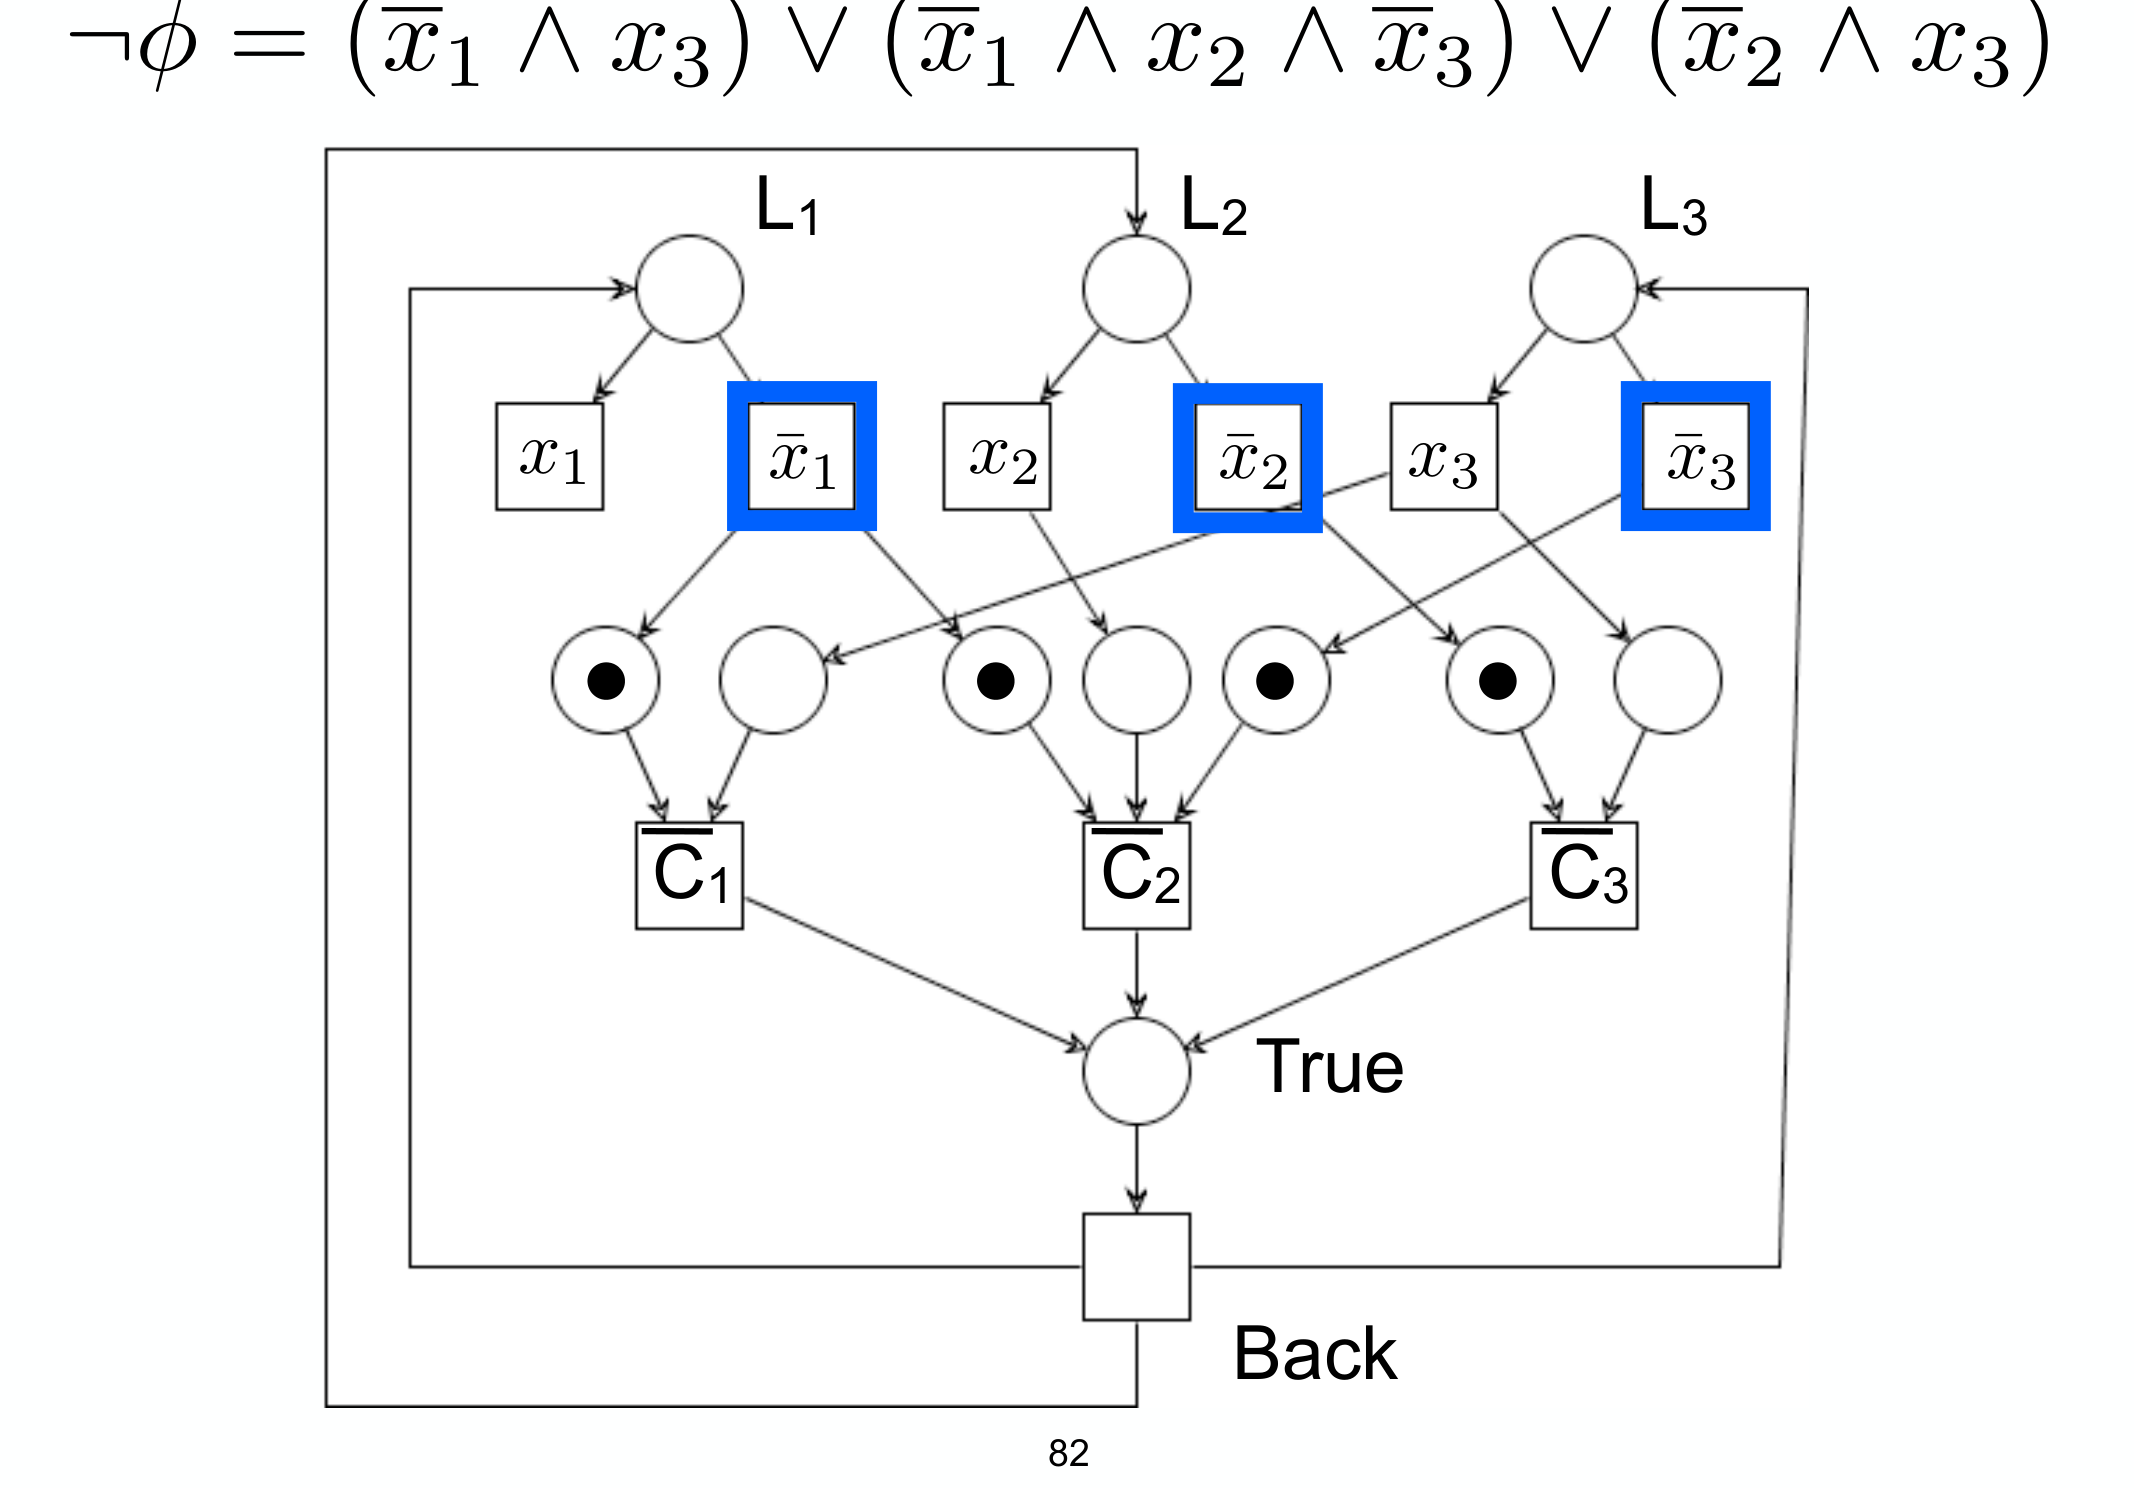
\includegraphics[width=0.74\linewidth,height=0.34\textheight,keepaspectratio]{images/17-free-choice_p82_sat-net.png}
\caption{Il net di una formula. \textbf{Fissare un'assegnazione} = scegliere, per ogni variabile, se scattare $x_i$ o $\bar{x_i}$ (scelta free-choice sul place $L_i$). Se l'assegnazione soddisfa $\neg\varphi$, qualche clausola-transition $\overline{C_i}$ resta bloccata e \textbf{Back diventa dead} $\rightarrow$ net non-live.}
\end{figure}

\begin{boxwarning}{Conseguenza principale}
Decidere la liveness di un free-choice system è \textbf{NP-complete}. L'algoritmo deterministico dovrebbe esplorare tutti i $2^{|P|}$ sottoinsiemi di place. \textbf{Non esiste} (a oggi) un algoritmo polinomiale per la sola liveness — \textbf{a meno che P = NP}.
\end{boxwarning}

\section{\texorpdfstring{Complessità 2: liveness + boundedness è polinomiale (Rank Theorem)}{Complessità 2: liveness + boundedness è polinomiale (Rank Theorem)}}

Ed ecco la sorpresa. Se si chiede \textbf{liveness E boundedness insieme} (esattamente ciò che serve per la \hyperref[ch:12]{soundness}: $N$ sound $\iff$ $N^\star$ live e bounded), il problema diventa \textbf{polinomiale}. Serve prima la nozione di \textbf{cluster}.

\begin{boxdefinition}{Cluster}
Il \textbf{cluster} di un nodo $x$, scritto $[x]$, è il più piccolo insieme tale che: 1. $x \in [x]$; 2. se un \textbf{place} $p \in [x]$, allora $p\bullet \subseteq [x]$ (tutte le sue transizioni uscenti); 3. se una \textbf{transition} $t \in [x]$, allora $\bullet t \subseteq [x]$ (tutti i suoi place entranti).

Intuitivamente si "chiude" alternando: da un place prendi le transizioni che ne escono, da una transizione i place che vi entrano. I cluster \textbf{partizionano} i nodi della rete; $C_N$ è l'insieme dei cluster.
\end{boxdefinition}

\begin{figure}[!htb]
\centering
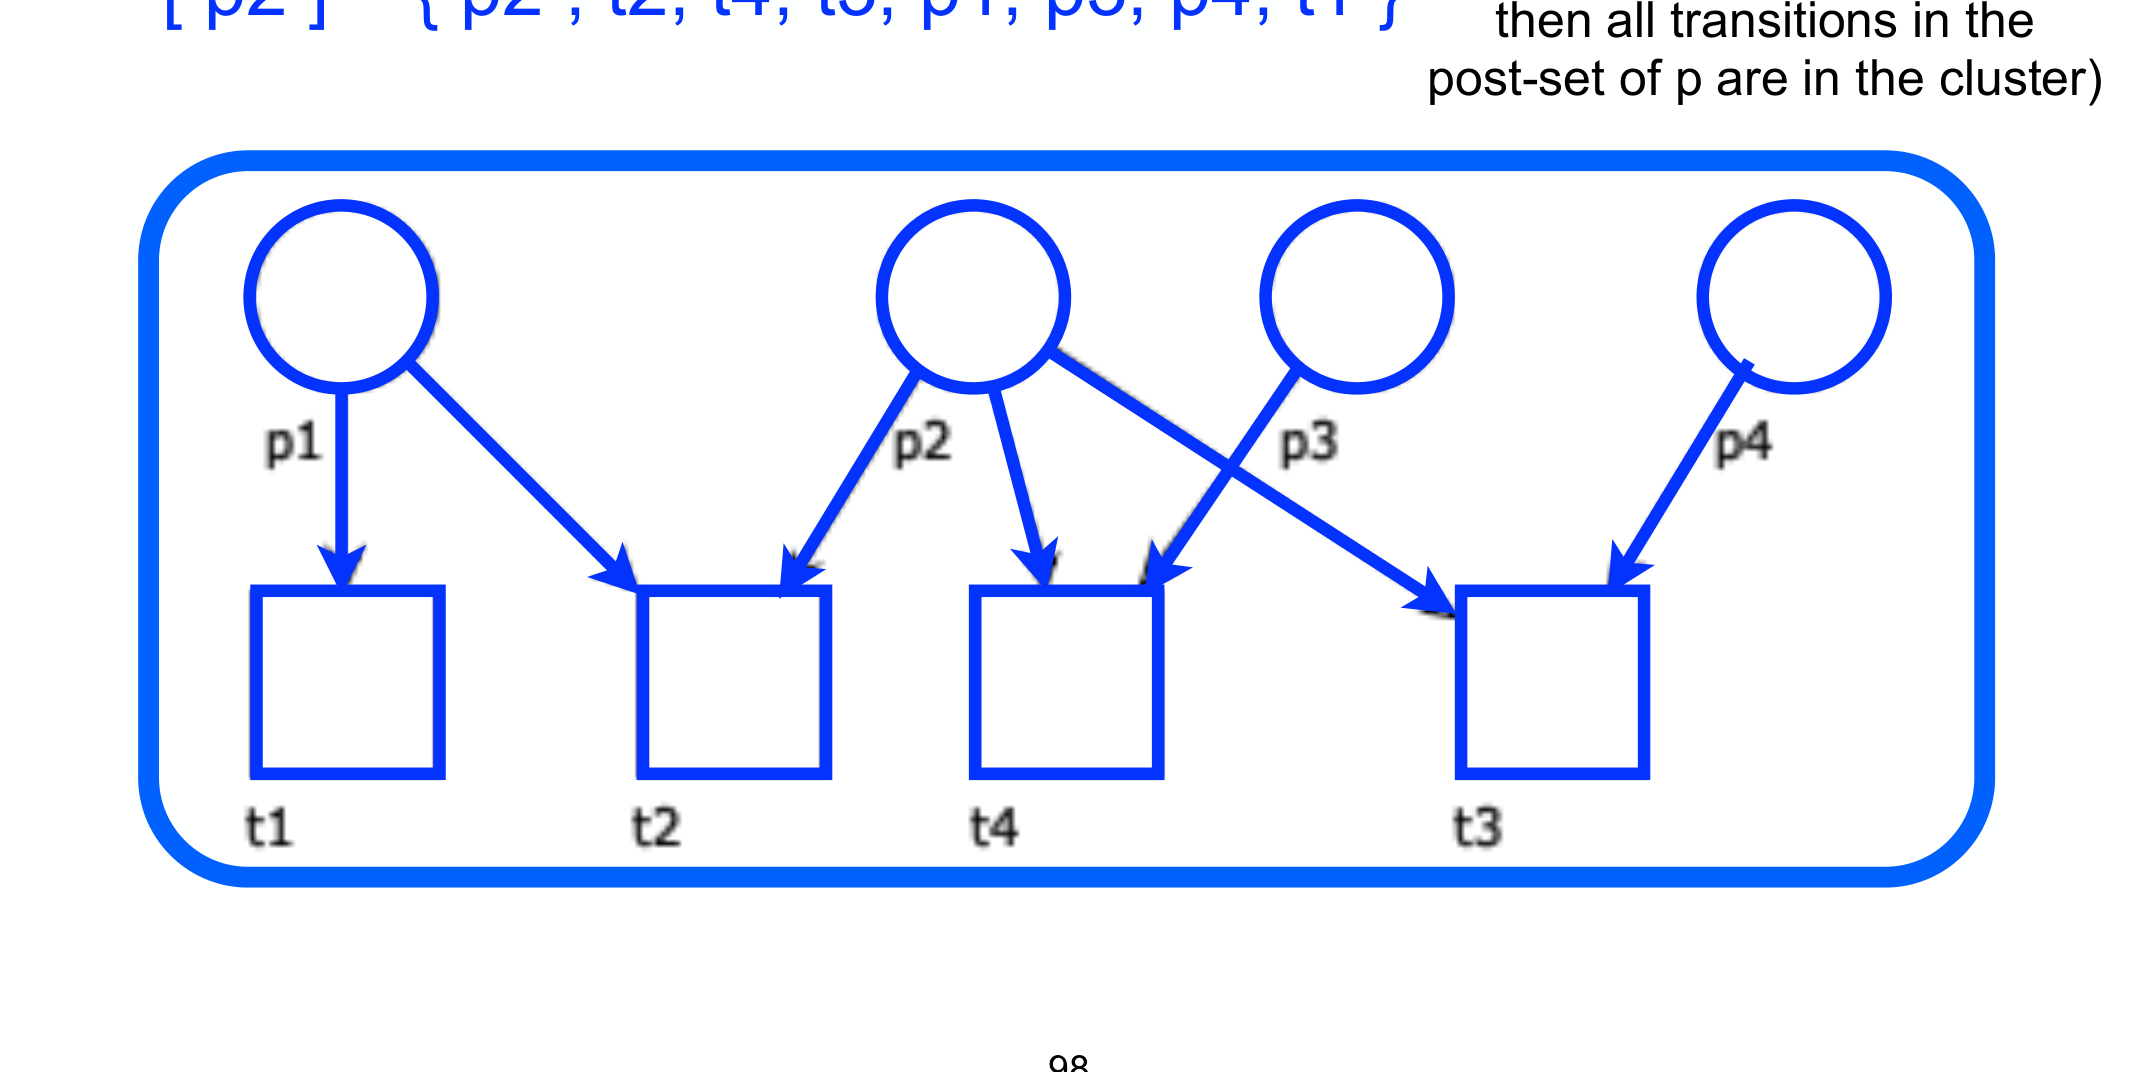
\includegraphics[width=0.74\linewidth,height=0.34\textheight,keepaspectratio]{images/17-free-choice_p98_cluster.png}
\caption{Costruzione di $[p_2]$: si alterna "place $\rightarrow$ sue transizioni uscenti" e "transizione $\rightarrow$ suoi place entranti" fino a chiusura. In un free-choice, un cluster è una "zona di scelta libera".}
\end{figure}

\begin{boxtheorem}{Rank Theorem (risultato principale, dim. omessa)}
Un free-choice system $(P,T,F,M_0)$ è \textbf{live e bounded} $\iff$ valgono tutte: 1. ha almeno un place e una transition; 2. è \textbf{connesso}; 3. $M_0$ marca \textbf{ogni proper siphon}; 4. ha un \textbf{S-invariant positivo} (tutte componenti $>0$); 5. ha un \textbf{T-invariant positivo}; 6. $\text{rank}(N) = |C_N| - 1$ (il rango della \hyperref[ch:11]{matrice di incidenza} è il numero di cluster meno uno).
\end{boxtheorem}

Il punto cruciale è che \textbf{ognuna} di queste sei condizioni si verifica in \textbf{tempo polinomiale}:

\begin{itemize}
\item connessione, invarianti positivi e rango: algebra lineare / visita del grafo, tutti poly;
\item "$M_0$ marca ogni proper siphon" si controlla calcolando il \textbf{massimo siphon non marcato} partendo dai place vuoti e togliendo iterativamente i place che violano la condizione: se resta vuoto, ogni proper siphon è marcato. Poly.
\end{itemize}

\begin{boxtip}{Il contrasto (take-home)}
\begin{itemize}
\item \textbf{Liveness da sola} su free-choice $\rightarrow$ \textbf{NP-complete} (riduzione da SAT).
\item \textbf{Liveness + boundedness} su free-choice $\rightarrow$ \textbf{polinomiale} (Rank Theorem).
\end{itemize}

Aggiungere un vincolo (la boundedness) \emph{semplifica} il problema invece di complicarlo! E poiché la soundness di un workflow net è proprio "$N^\star$ live e bounded", per i workflow net \textbf{free-choice} la soundness si decide in \textbf{tempo polinomiale}. È la giustificazione teorica del perché tool come WoPeD funzionano bene sui processi reali (che sono quasi sempre free-choice).
\end{boxtip}

\section{\texorpdfstring{Recap}{Recap}}

\begin{boxabstract}{Free-choice net: il quadro}
\begin{itemize}
\item \textbf{free-choice}: pre-set delle transizioni disgiunti o uguali $\rightarrow$ la scelta è \emph{libera}, non influenzata dal resto;
\item place-liveness $\iff$ liveness;
\item \textbf{non-live} $\iff$ esiste un proper siphon il cui trap massimale è non marcato (\textbf{Commoner});
\item decidere la sola \textbf{liveness} è \textbf{NP-complete};
\item decidere \textbf{liveness + boundedness} è \textbf{polinomiale} (\textbf{Rank Theorem}) $\rightarrow$ soundness poly per WF net free-choice.
\end{itemize}
\end{boxabstract}

Con questi strumenti chiudiamo l'analisi strutturale del singolo processo. La prossima lezione estende il discorso ai \textbf{workflow system}, dove più processi comunicano — riprendendo il problema "sound + sound $\neq$ sound" visto con Buyer/Reseller. $\rightarrow$ \hyperref[ch:18]{18 — Workflow Systems}